\documentclass[border=7pt]{standalone}
\usepackage{tikz}
\begin{document}
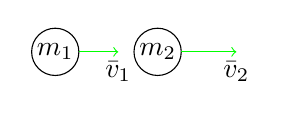
\begin{tikzpicture}
  \draw (4.4,-2) circle [radius=0.3]  node {$m_1$};
  \draw (5.7,-2) circle [radius=0.3]  node {$m_2$};
  \draw [green, ->] (6,-2) -- (6.7,-2) node [black, right, below] {$\bar{v}_2$};
  \draw [green, ->] (4.7,-2) -- (5.2,-2) node [black, right, below] {$\bar{v}_1$};
\end{tikzpicture}
\end{document}
